%
% Cifradores de flujo autosincronizables, capítulo de antecedentes.
% Proyecto Lovelace.
%

\subsection{Autosincronizables}

En esta clasificación se engloban a aquellos cifrados cuyo flujo de llave es
resultado de la propia llave original y de cierto número previo de dígitos
cifrados. Las ecuaciones que describen su comportamiento son las siguientes.

\begin{equation}
  \label{asinc:cambio_de_estado}
  e_{i+1} = (c_{i - t}, c_{i - t + 1}, \dots, c_{i - 1})
\end{equation}

\begin{equation}
  \label{asinc:flujo_de_llave}
  l_i = g(e_i, L)
\end{equation}

\begin{equation}
  \label{asinc:funcion_de_salida}
  c_i = h(l_i, m_i)
\end{equation}

La notación es la misma que en las ecuaciones \ref{sinc:cambio_de_estado},
\ref{sinc:flujo_de_llave} y \ref{sinc:funcion_de_salida}. En este caso, el
próximo estado depende de $ t $ (el tamaño de la ventana) dígitos cifrados
anteriormente. En la figura \ref{flujo_asincrono} se describe de manera
gráfica el proceso de cifrado y descifrado.

\begin{figure}[H]
  \centering
  \begin{subfigure}{0.45\textwidth}
    \begin{center}
      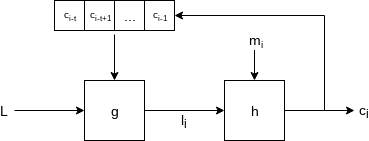
\includegraphics[width=0.9\linewidth]
        {contenidos/antecedentes/cifrados_de_flujo/diagramas/asincrono_cifrado.png}
      \caption{Cifrado.}
    \end{center}
  \end{subfigure}
  \begin{subfigure}{0.45\textwidth}
    \begin{center}
      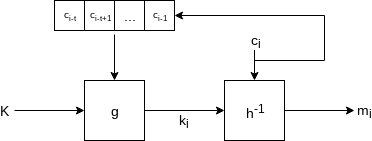
\includegraphics[width=0.9\linewidth]
        {contenidos/antecedentes/cifrados_de_flujo/diagramas/asincrono_descifrado.png}
      \caption{Descifrado.}
    \end{center}
  \end{subfigure}
  \caption{Esquema general de un cifrado de flujo autosincronizable.}
  \label{flujo_asincrono}
\end{figure}

En una antítesis de la categoría anterior, el nombre de esta indica que no es
necesario que el emisor y el receptor estén sincronizados: si se llegan a
perder bits en la transmisión, el esquema es capaz de autosincronizarse, pues
el flujo de la llave depende de cierto número de bits anteriores. A esta
categoría también se le conoce como «asíncrona».

La propagación de los errores depende del tamaño de ventana (el número $ t $
de bits previos utilizados para calcular la próxima llave), si se modifica un
bit, entonces los próximos $ t $ serán incorrectos.
